\everymath{\displaystyle}
%\documentclass[pdftex,a4paper]{article}
\documentclass[a4paper]{article}
%%classes: article, report, book, proc, amsproc

%%%%%%%%%%%%%%%%%%%%%%%%
%% Misc
% para acertar os acentos
\usepackage[brazilian]{babel}
%\usepackage[portuguese]{babel}
% \usepackage[english]{babel}
% \usepackage[T1]{fontenc}
% \usepackage[latin1]{inputenc}
\usepackage[utf8]{inputenc}
\usepackage{indentfirst}
\usepackage{fullpage}
% \usepackage{graphicx} %See PDF section
\usepackage{multicol}
\setlength{\columnseprule}{0.5pt}
\setlength{\columnsep}{20pt}
%%%%%%%%%%%%%%%%%%%%%%%%
%%%%%%%%%%%%%%%%%%%%%%%%
%% PDF support

\usepackage[pdftex]{color,graphicx}
% %% Hyper-refs
\usepackage[pdftex]{hyperref} % for printing
% \usepackage[pdftex,bookmarks,colorlinks]{hyperref} % for screen

%% \newif\ifPDF
%% \ifx\pdfoutput\undefined\PDFfalse
%% \else\ifnum\pdfoutput > 0\PDFtrue
%%      \else\PDFfalse
%%      \fi
%% \fi

%% \ifPDF
%%   \usepackage[T1]{fontenc}
%%   \usepackage{aeguill}
%%   \usepackage[pdftex]{graphicx,color}
%%   \usepackage[pdftex]{hyperref}
%% \else
%%   \usepackage[T1]{fontenc}
%%   \usepackage[dvips]{graphicx}
%%   \usepackage[dvips]{hyperref}
%% \fi

%%%%%%%%%%%%%%%%%%%%%%%%


%%%%%%%%%%%%%%%%%%%%%%%%
%% Math
\usepackage{amsmath,amsfonts,amssymb}
% para usar R de Real do jeito que o povo gosta
\usepackage{amsfonts} % \mathbb
% para usar as letras frescas como L de Espaco das Transf Lineares
% \usepackage{mathrsfs} % \mathscr

% Oferecer seno e tangente em pt, com os comandos usuais.
\providecommand{\sin}{} \renewcommand{\sin}{\hspace{2pt}\mathrm{sen}}
\providecommand{\tan}{} \renewcommand{\tan}{\hspace{2pt}\mathrm{tg}}

% dt of integrals = \ud t
\newcommand{\ud}{\mathrm{\ d}}
%%%%%%%%%%%%%%%%%%%%%%%%

\title{Avaliação Parcial da disciplina de Metodologia Científica}
\date{}
\author{Docente: Felipe Figueiredo\\
  \url{prof.felipefigueiredo@gmail.com}\\
  \url{http://sites.google.com/site/proffelipefigueiredo}
}
\begin{document}
\maketitle
\abstract{Nesta avaliação parcial, os alunos deverão redigir um texto
  dissertativo que simule um projeto de pesquisa. Aqui estão gráficos
  que descrevem um conjunto de dados preliminar, como se obtidos em um
  projeto piloto. Caberá aos alunos (a) formular um problema de
  pesquisa baseado nesses dados preliminares, (b) indicar que outros
  tipos de dados deverão ser coletados para atender às questões
  levantadas, (c) justificar suas escolhas, preferencialmente com
  algumas referências bibliográficas.

  Obs: Os dados preliminares aqui contidos são altamente fictícios,
  portanto não há pergunta ou resposta correta nesta avaliação, apenas
  bons argumentos. Confronte-os com suas expectativas e intuição.}

\newpage

%%%%%%%%%%%%%%%%%%%%%%%%
%% Título e cabeçalho
%\noindent\parbox[c]{.15\textwidth}{
\includegraphics[width=.15\textwidth]{logo}}\hfill
\parbox[c]{.825\textwidth}{\raggedright%
  \sffamily {\LARGE

Metodologia Científica

Avaliação Parcial

\par\bigskip}
{Prof: Felipe Figueiredo\par}
{\url{http://sites.google.com/site/proffelipefigueiredo}\par}
}

Versão: \verb|YYYYMMDD|

%%%%%%%%%%%%%%%%%%%%%%%%


%%%%%%%%%%%%%%%%%%%%%%%%

\section{Objetivos}
O objetivo primário desta avaliação é proporcionar ao discente uma
primeira oportunidade de redigir um anteprojeto, seguindo normas
adequadas à pesquisa científica, e ao programa de Pós-Graduação. Para
tal, serão avaliados a clareza na exposição textual, e a exposição do
material, seguindo os padrões estabelecidos de formatação de página,
parágrafo, referências e demais elementos.

O objetivo secundário desta avaliação é estimular tanto a criatividade
acadêmica como a habilidade de formulação de problemas.

\section{Contexto}

{\bf Situação fictícia:} sabemos pouco sobre a relação entre a
obesidade e o risco de doenças cardíacas. Cabe a vocês propor um
projeto para verificar esta relação!

Estudos recentes parecem indicar que a obesidade é um fator de risco
para doenças cardiovasculares. A métrica usada nestes estudos como
preditora para esse risco, é a medida de Circunferência Abdominal
(CA).

O pesquisador John Doe, deste instituto de pesquisa, está sem tempo
para estudar essa relação, mas conseguiu coletar alguns dados
preliminares de CA de alguns voluntários e plotou alguns gráficos
descritivos destes dados. Nessa análise exploratória de dados, ele
plotou um gráfico de dispersão (Figura \ref{fig:dispersao}), um
histograma (Figura \ref{fig:histograma}) e um boxplot (Figura
\ref{fig:boxplot}). Ele espera que estes gráficos sejam úteis para
você formular um projeto de pesquisa.

John Doe dispõe de amplos recursos e infra-estrutura de pesquisa em
seu laboratório, e está disposto a oferecer seus recursos para que
vocês desenvolvam um projeto de pesquisa interessante. Vocês poderão
usar o laboratório de John Doe, desde que ele seja incluído como
co-autor (último nome na lista de autores).

\begin{figure}[h]
  \centering
  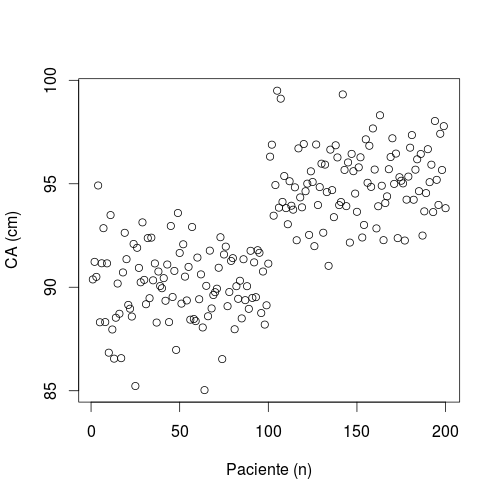
\includegraphics[width=.5\textwidth]{dispersao}
  \caption{Gráfico de dispersão da Circunferência Abdominal (CA) de
    cada paciente (homens adultos).}
  \label{fig:dispersao}
\end{figure}

\begin{figure}[h]
  \centering
  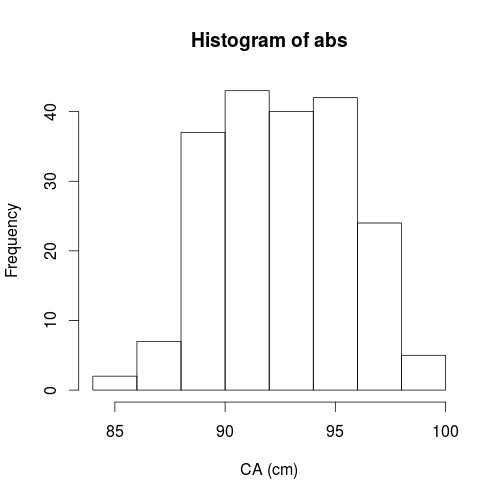
\includegraphics[width=.5\textwidth]{histograma}
  \caption{Histograma de frequências da Circunferência Abdominal (CA)
    de homens adultos.}
  \label{fig:histograma}
\end{figure}

\begin{figure}[h]
  \centering
  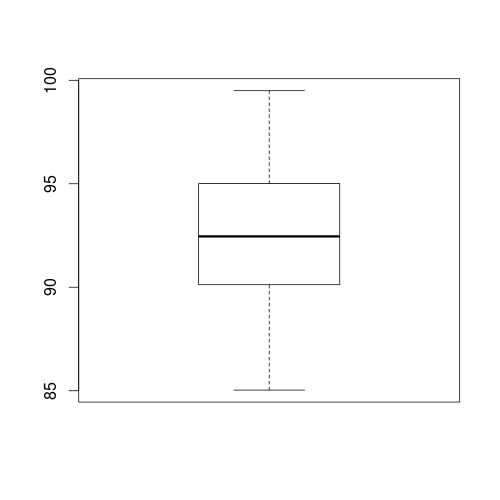
\includegraphics[width=.5\textwidth]{boxplot}
  \caption{Boxplot da Circunferência Abdominal (CA) de homens
    adultos.}
  \label{fig:boxplot}
\end{figure}

% \begin{itemize}
% \item objetivo: os alunos devem, já sabendo a resposta por experiência
%   própria, elaborar um projeto fictício para testar essa pergunta.
% \item premissa: o dataset é um preliminar, de um estudo piloto, que
%   servirá de base para o texto.
% \item Devem pensar em como formular a hipótese, e descrever os
%   resultados preliminares.
% \end{itemize}

\section{Projeto}

Tomando como base os dados preliminares do projeto piloto de John Doe,
vocês devem formular:

\begin{itemize}
\item um problema de pesquisa (pergunta)
\item hipóteses
\item um plano de execução da pesquisa
\end{itemize}

Este projeto deve ser redigido conforme as normas desta instituição
para o seminário de acompanhamento discente (qualificação). A
descrição deste formato está na página da instituição. Quaisquer
dúvidas quanto ao formato podem ser tiradas com o docente.

Sugere-se que os grupos dividam a elaboração do projeto acompanhando
as aulas, redigindo um rascunho inicial de cada parte do documento
progressivamente, seguindo as recomendações oferecidas nas aulas. Este
rascunho inicial de cada parte (Introdução, Metodologia, Resultados,
\ldots) deve ser revisto periodicamente, para o refinamento da
qualidade textual.

Após a entrega do projeto textual, o grupo deverá apresentar um
seminário onde defenderá os argumentos apresentados no projeto. A
avaliação desta disciplina é composta tanto pelo projeto quanto pela
apresentação, com pesos iguais.

\section{Seções do projeto}

\subsection{Seções requeridas}

Cada seção do projeto deve iniciar em uma nova página. O projeto deve
conter minimanente os seguintes ítens:

\begin{itemize}
\item Justificativa (sugestão 1 página)
\item Revisão da literatura (sugestão 1--2 páginas)
\item Objetivos (1 página)
\item Metodologia (sugestão 1 página)
\item Cronograma de atividades (sugestão 1 página)
\item Referências bibliográficas (sugestão 1 página)
\end{itemize}

\subsection{Cronograma}

O projeto deve incluir um cronograma, descrevendo metas para um plano
a ser executado em dois anos. O cronograma do projeto deve incluir:

\begin{itemize}
\item Revisão bibliográfica inicial (sugestão 2--6 meses)
\item Coleta de dados (sugestão 12--18 meses)
\item Análise de dados (sugestão 1--3 meses)
\item Apresentação de resultadoos preliminares em seminário/congresso
  (opcional)
\item Revisão bibliográfica complementar e discussão dos resultados
  (sugestão 2--6 meses)
\item Redação do relatório principal (sugestão 2--4 meses)
\item Redação de artigo para submissão em periódico científico
\end{itemize}

Os ítens dos cronograma podem se sobrepor caso seja necessário, sempre
observando a viabilidade da sobreposição de tarefas\footnote{Observe
  que estas sugestões são para este projeto fictício, e não uma regra
  para projetos de Mestrado.}.

% \section{Problema}

% \begin{itemize}
% \item existe uma correlação entre a circunferência abdominal e doença
%   cardíaca?
% \end{itemize}

\end{document}
